\documentclass[10pt,twocolumn,letterpaper]{article}

\usepackage{cvpr}
\usepackage{times}
\usepackage{epsfig}
\usepackage{graphicx}
\usepackage{amsmath}
\usepackage{amssymb}
\usepackage{caption}
\usepackage{subcaption}
\usepackage{xcolor}

% Include other packages here, before hyperref.

% If you comment hyperref and then uncomment it, you should delete
% egpaper.aux before re-running latex.  (Or just hit 'q' on the first latex
% run, let it finish, and you should be clear).
\usepackage[breaklinks=true,bookmarks=false]{hyperref}

\cvprfinalcopy % *** Uncomment this line for the final submission

\def\cvprPaperID{****} % *** Enter the CVPR Paper ID here
\def\httilde{\mbox{\tt\raisebox{-.5ex}{\symbol{126}}}}

\def\ti{\mathbf{t}_i}
\def\si{\mathbf{s}_i}

\newcommand{\ignore}[1]{}
\DeclareMathOperator*{\argmin}{arg\,min}

\newcommand{\TODO}[1]{
	{\bfseries\colorbox{red}{\color{white}TODO: #1}}
}

% Pages are numbered in submission mode, and unnumbered in camera-ready
%\ifcvprfinal\pagestyle{empty}\fi
\setcounter{page}{1}
\begin{document}

%%%%%%%%% TITLE
\title{Stereo Analogies}

\author{Alexandre Kaspar\\
\\
{\tt\small akaspar@csail.mit.edu}
}
%\thispagestyle{empty}

\twocolumn[{%
\renewcommand\twocolumn[1][]{#1}%
\maketitle
\begin{center}
	\centering
	\includegraphics[width=0.7\textwidth]{figures/teaser2}
	\captionof{figure}{Automatic synthesis of stereoscopic frames using a large set of frames.}
	\label{fig:teaser}
\end{center}
}]

%%%%%%%%% ABSTRACT



\begin{abstract}
We explore image analogies applied to stereoscopic data synthesis by leveraging an external source of stereo data instead of estimating scene motion or using geometric cues to infer depth / disparity.
We present our approach to work with a large database of such images and provide insights on disparity computation given our findings.
\end{abstract}

%%%%%%%%% BODY TEXT


\section{Introduction}

Topic: stereo synthesis.

Related:
\begin{itemize}
	\item stereo disparity (even optical flow != motion flow)
	\item scene synthesis
	\item texture / style transfer
	\item nearest neighbor computation $\to$ patch match
	\item scene recognition $\to$ find patches in multiple images
\end{itemize}

Texture is important for photorealistic depiction as it provides a succinct description of surface properties and details which can be hard to specify otherwise.
It is extensively used in computer graphics for augmenting coarse geometric models with fine surface details, while imaging softwares such as Photoshop have been using it to provide hole filling, seamless blending and other tools where the impression of detail matters.

%-------------------------------------------------------------------------
\subsection{Texture Synthesis}

As it can be difficult to acquire textures that fit the resolution and boundary constraints of a specific modeling task, one might be interested in automatically synthesizing texture.
Algorithms for texture synthesis include parametric approaches such as \textbf{procedural texture} models \cite{Ebert02, Musgrave93, Worley96} based on particular texture models (e.g.\;wood, cloud, ground, fire), as well as exemplar-based methods that have been very popular recently.
While many texture models have been explored for exemplar-based synthesis \cite{Heeger95}, we focus on the Markov Random Field methods that have produced the most impressive results so far (which we briefly present here, see \cite{Wei09} for more details).

\textbf{Pixel-based} methods \cite{Efros99} grow textures one pixel at a time by selecting exemplar patches that match the window around the newly synthesized pixel.
Different accelerations have been proposed such as fixed neighborhoods and scanline processing \cite{Wei00}, $k$-coherence \cite{Tong02} and eventually led to \textbf{patch-based} methods \cite{Praun00, Efros01, Liang01, Kwatra03} that directly copy full patches.

Then came \textbf{optimization-based} methods \cite{Kwatra05} that grow the texture as a whole by minimizing a patch energy
\begin{equation}
	\sum_i d(\ti, \si)
	\label{eq:patch_energy}
\end{equation}
where $\ti$ are patches of our synthesized target, $\si$ are the corresponding patches in the exemplar and $d(\cdot)$ is a patch distance such as the sum of squared differences.

Further controllability has been introduced with the use of extra feature channels \cite{Ashikhmin01, Matusik05, Lefebvre06, Lu07}.

\subsection{Applications}

Many of the aforementioned methods have applications outside of simple texture synthesis.
For example, 2D patches have been extended into 3D patches for solid texture synthesis \cite{Wei02, Kopf07, Dong08} or extended with a temporal dimension for video textures \cite{Schodl00, Schodl02, Agarwala05} and spatio-temporal video texture synthesis \cite{Kwatra03, Wexler07}.
Editing tools have been developed using texture-based methods such as style transfer \cite{Efros01, Hertzmann01} and image completion \cite{Bertalmio00, Drori03, Hays07} that have then been used for geometry \cite{Bhat04, Zhou06} and shape synthesis \cite{Rosenberger09}.

\section{Overview}
\texttt{Texture Synthesis using Patch Match}

We present here the recent work of Darabi \cite{Darabi12} - Image Melding - that builds upon Texture Optimization \cite{Kwatra05} with the addition of two new components: the Patch Match algorithm \cite{Barnes09} for fast nearest neighbor search, and the integration of gradient blending to propagate boundary constraints for more efficient image editing \cite{Agarwala04}.

The minimization of Equation \ref{eq:patch_energy} is done by alternating between the two following steps:
\begin{itemize}
	\setlength{\itemsep}{4pt}
  \setlength{\parskip}{0pt}
  \setlength{\parsep}{0pt}
	\item \textbf{Nearest Neighbor Search}: optimize for $\si$ with $\ti$ fixed, which corresponds to finding the nearest neighbors $\si$ of patches $\ti$ ($\ti$ in result, $\si$ in exemplar)
	\item \textbf{Vote}: given the fixed nearest neighbors $\si$, optimize for the patches $\ti$ in the target result, which corresponds to averaging overlapping patches to get the desired pixels
\end{itemize}

This is done iteratively, using a scale pyramid from coarse to fine scale, until convergence or a given number of steps at each level of the pyramid.
Image Melding also generates gradient information during the voting process and blends it in a third step using the work of \cite{Bhat08}:
\begin{itemize}
	\item \textbf{Screened Poisson Equation}: for the best pixel intensity given current pixel intensities and gradients
\[
	T^*=\argmin_{T} \sum (T - \overline{T})^2 + \lambda \| \nabla T - \overline{\nabla T}\|^2
\]
where $\overline{T}$ and $\overline{\nabla T}$ are the averaged pixel intensities and gradients from the voting step, and $\nabla T$ is the gradient operator applied to the unknown best pixel intensities.
\end{itemize}

%-------------------------------------------------------------------------
\texttt{Project Proposal}

Given the plethora of applications using texture synthesis and the many variations we presented, we propose a new target for exemplar-based texture synthesis: synthesizing stereo-view video from a single-view video stream (for example to view it in 3D).

\subsection{Traditional stereo methods}

The traditional multi-view approach consist in partially modeling the 3D environment such as with Hyper-lapse videos \cite{Kopf14} or stereo reconstruction \cite{Seitz06}. A naive approach for stereo synthesis would therefore be to use video frame correspondences to register the camera path and content geometry, which would provide a way to synthesize stereo-view video.

\subsection{Our approach}

Since the many steps required by multi-view reconstruction do not always work well and accumulate errors, we propose a much simpler approach based on texture synthesis to generate the second stream of a stereo-view video stream using patch correspondences.

The basic idea consists of having a set of true stereo videos (seemingly available \cite{Corrigan10, Smolic10}) as exemplar frames.
Given the pair of true streams $L$ and $R$ (left and right image streams) and a new single-view stream $L'$, we can synthesize its corresponding part $R'$ by
\begin{enumerate}
	\setlength{\itemsep}{4pt}
  \setlength{\parskip}{0pt}
  \setlength{\parsep}{0pt}
	\item Finding the nearest neighbor patches of $L'$ in $L$
	\item Using the corresponding patches in $R$ for $R'$
\end{enumerate}
which corresponds to image analogies \cite{Efros01, Hertzmann01} applied to stereo video streams.

The potential new problems to deal with include
\begin{itemize}
	\setlength{\itemsep}{4pt}
  \setlength{\parskip}{0pt}
  \setlength{\parsep}{0pt}
	\item Dealing with time coherence efficiently (either using 3D spatio-temporal patches or per-frame 2D patches with some extra coherence constraint)
	\item Retrieving patches from multiple exemplars \cite{Barnes11, Hu13} (i.e. multiple frames and a collection of video streams)
\end{itemize}

Framework:
\begin{itemize}
	\item NNF from A' to A
	\item Stereo transfer (style, difference, disparity, etc.)
	\item Multi-scale pyramid / Laplacian pyramid
\end{itemize}

\section{Implementation}

We provide details about the nearest neighbor computation with Patch Match~\cite{Barnes09} and its multiple exemplar version Patch Web~\cite{Barnes11}.
Finally, we mention details about the different transfer strategies and especially how we got the frame disparity.

Along this section, we assume that the input frame $L'$ is the left frame and we find a k-NNF from its patches to patches within the left images $L$ of our database. The database also contains the corresponding right frames $R$ and our goal is to eventually synthesize $R'$ from $L'$.

\subsection{Patch Match}

Given an input image $A$ made of overlapping $N\times N$ patches $\{\ti\}$, we want to find the closest patches $\{\si\}$ in an image $B$, i.e.
\begin{equation}
	\si^{*} = \argmin_{\si \in B} d(\ti, \si)
\end{equation}
for some distance $d(\cdot)$, usually the sum of squared differences or a L2 norm.

A naive brute-force computation would enumerate all possible patch assignments and find the best one.
However, this is computationally unreasonnable given the context of our large high resolution image database.

Patch Match~\cite{Barnes09} is a fast approximate nearest neighbor algorithm specifically tuned for image patches and thus our problem.
It is based on the \emph{coherence assumption}, namely that, while patches mapped from $A$ to $B$ can be mapped everywhere in $B$, nearby patches in $A$ are usually mapped together in $B$.

\begin{figure}[ht]
\centering
	\begin{subfigure}[t]{0.155\textwidth}
		\includegraphics[width=\textwidth]{figures/propagation_text2}
		\caption{Propagation}
	\end{subfigure}
	\begin{subfigure}[t]{0.155\textwidth}
		\includegraphics[width=\textwidth]{figures/randsearch_text}
		\caption{Random search}
	\end{subfigure}
	\begin{subfigure}[t]{0.155\textwidth}
		\includegraphics[width=\textwidth]{figures/voting_text}
		\caption{Voting}
	\end{subfigure}
   \caption{The main components of texture synthesis using Patch Match.}
\label{fig:texsynth_patchmatch}
\end{figure}

The algorithm proceeds in scanline-order from an initial guess of the nearest neighbor assignments $\{\ti \to \si\}$ and tries new candidate nearest neighbor patches using two main operations:
\textbf{propagation} which tries to propagate the result of neighboring mappings, and 
\textbf{random search} that randomly samples patches in an exponentially decreasing window (see illustrations in Figure~\ref{fig:texsynth_patchmatch}).

Given these patch assignments, we can transfer localized data.
This last step involves different strategies which we details in Section~\ref{sec:transfer}. 
All of them are forms of \emph{voting} since by having $N\times N$ patches, each of the pixels of our output image technically has as many overlapping patches to choose from.
The usual voting consist of averaging the overlapping pixels which minimizes the average L2 distance.

\paragraph{Extensions}
The Patch Match algorithm has been extended in several ways \cite{Barnes10} including the sampling of rotations, scales and mirrored patch spaces, the use of gain and bias adjustment, a $k$-NN version of the algorithm as well as extra operations (uniform sampling, enrichment and binning).

Application-specific variants of voting have been explored such as Meanshift \cite{Wexler07}, Histogram weighting \cite{Kopf07} as well as Bidirectional Similarity \cite{Simakov08}.

\subsection{Patch Web}
Extending the algorithm to multiple exemplars is straightforward: patches now also contain the new variable exemplar index they come from.
Furthermore, to improve performance, additional sampling strategies have been designed~\cite{Barnes11}:

\paragraph{Uniform sampling} searches over all patches of all exemplars (this is very similar to random search, with a new exemplar dimension to search through).

\paragraph{Enrichment} finds new candidates by looking at what patches we are mapped to, are mapped to (forward enrichment $f$) or to use the reverse mapping (backward enrichment $f^{-1}$) similarly.
Variants consider multiple hops such as $f^2$, $f^3$, $\dots$ or $f^{-2}$, etc.

Given a $k$-NNF, one can use enrichment with the $k$ candidates or a subset, leading to many potential variants.

\paragraph{Binning} divides the patches into bins similarly to what a histogram would do, and samples patches from the bin corresponding to the patch we sampling for.
To bin patches, usually a lower-dimension space is used ($N\times N$ patches with $C$ channels have $CN^2$ dimensions) by computing PCA.

Recent alternatives~\cite{He12} use Walsh-Hadamard Transform bases~\cite{Hel05} instead of PCA.

Our implementation contains all the aforementioned candidate lookups but binning because of the high memory requirement that makes it harder to implement wisely (other strategies require basically no additional memory storage).

\subsection{Stereo Transfer}
\label{sec:transfer}
Armed with an effective multiple exemplar k-NNF computation, there remains to transfer the stereoscopic information and synthesize our right frame.

\begin{enumerate}
	\item Compute constrained k-NNF from left to right
	\item Vote disparity
\end{enumerate}

Multiple voting strategies are possible:
\begin{itemize}
	\item Merge k-NNF into 1-NNF and then take naive patch shift as disparity
	\item Compute average disparity of $k \times N \times N$ overlapping patches
	\item Compute it with Mean-Shift
\end{itemize}

\TODO{Use patches with 5 channels: L, a, b, x, y}
\TODO{location of patch matters for disparity}

\TODO{talk about the missing "binning"}

\TODO{mention halfway domain}


\section{Results}

Nice figures and evaluation.

No need for high resolution~\cite{Sawhney01, Stelmach00}

\TODO{Show results for transfers = patch, difference, disparity}
\TODO{Show disparity computations using our PM}
\TODO{Mention PM-Forest}
\TODO{Show convergence results for different candidate strategies}


\section{Conclusion}

The results in Table~\ref{tbl:results} surprinsingly show that incrementally building the NNF is usually detrimental.
This might be because of the poor convergence of PatchMatch using multiple exemplars and the algorithm getting stuck in local energy minima at the lower scales (although one should expect pyramidal computation to help against these).

For \emph{smooth frames}, whole patch and patch difference transfer both tend to perform better than disparity transfer in our results.
For \emph{high variation frames} (especially the ones from Elephant Dreams, prefixed \texttt{ed\_}), disparity transfer appears more effective.

\paragraph{Occlusions} produce artifacts at the boundary of object in each of the stereoscopic transfer strategies we devised.
High variation images might not suffer so much from this because of the high visual clutter.

In general, complicated heuristics could be devised to solve this.
However we envision to use a different approach that consists of working with a half-way domain between the left and right frames instead of deliberately choosing to work on the left side.
Indeed, why should we work with one side and not the other? How should we merge both results if we were to work with both sides in parallel?
The nicer solution is to work with the half-way domain of~\cite{Liao14} which nicely interpolates occluded data.

\paragraph{Disparity} maps we computed with Classic-NL-Fast might be too low-resolution for our database and queries (see comparisons in Figure~\ref{fig:disp_results}).
We expect that the general poor results we achieved with disparity transfer are due to the bad quality of our disparity mappings.

\paragraph{Convergence} is still an issue and while patch propagation is the most effective patch update with uniform search, the most logical search strategy is that of binning which selects patches whose features are close to that of the considered patches, i.e. naturally good patches with low distances.
We mentioned that this is a complicated part to implement for memory reasons.
While the usual dimension reduction involves PCA, recent alternatives~\cite{He12} use Walsh-Hadamard Transform bases~\cite{Hel05} to produce the subspace much more efficiently.
We could then compute the subspace in a round-robin manner, keeping only the subspace of one image at a time, or sections of the subspace, etc.

Finally, these results are encouraging.
They hopefully tend to show that large sources of stereoscopic data might be leveraged for stereo image synthesis.


{\small
\bibliographystyle{ieee}
\bibliography{report}
}

\end{document}
